%\documentclass[12pt]{article}
\documentclass[11pt]{article}

\addtolength{\textwidth}{1.4in}
\addtolength{\oddsidemargin}{-0.5in}
\addtolength{\evensidemargin}{-0.5in}
%\addtolength{\topmargin}{-0.5in}
\addtolength{\topmargin}{-1.0in}
\addtolength{\textheight}{1.7in}
\newlength{\defbaselineskip}
\setlength{\defbaselineskip}{\baselineskip}

\usepackage{algorithm}
\usepackage{algpseudocode}
\usepackage{framed}
\usepackage{amssymb}
\usepackage{amsfonts}
\usepackage{amsmath}
%%% \usepackage{verbatim}
\usepackage{graphicx}
%\usepackage{caption}
%%\DeclareCaptionType{copyrightbox}
%\usepackage{subcaption}
\usepackage{url}
\usepackage{rotating}
\usepackage{multirow}
\usepackage{color}
\usepackage{xcolor}
%%\usepackage{enumitem}
\usepackage{paralist}

%\usepackage{subfig}
\usepackage{subfigure}

\usepackage{longtable} 
\usepackage{makecell}

\usepackage[multiple]{footmisc}
\usepackage[section]{placeins}

\usepackage{hyperref}
\hypersetup{
     colorlinks   = true,
     linkcolor    = blue,
     citecolor    = green
}

%-----------------------------------------------------------------------

\newcommand{\fix}[1]{\textcolor{red}{#1}}
\newcommand{\comment}[1]{\textcolor{blue}{#1}}
\newcommand{\awk}[1]{\textcolor{green}{#1}}

\newcommand{\argmin}{\text{argmin}}
\newcommand{\Probab}[1]{\mbox{}{\bf{Pr}}\left[#1\right]}
\newcommand{\Expect}[1]{\mbox{}{\bf{E}}\left[#1\right]}
\newcommand{\ExpectBracket}[1]{\mbox{}\langle#1\rangle}

% Here are two macros for comments.
\newcommand {\nred}[1]{{\color{red}\sf{[#1]}}}
\newcommand {\ngreen}[1]{{\color{green}\sf{[#1]}}}
\newcommand {\ncyan}[1]{{\color{cyan}\sf{[#1]}}}
\newcommand {\michael}[1]{{\color{red}\sf{[michael: #1]}}}
\newcommand {\charles}[1]{{\color{blue}\sf{[charles: #1]}}}
\newcommand {\serena}[1]{{\color{orange}\sf{[charles: #1]}}}

\usepackage[normalem]{ulem}



%-----------------------------------------------------------------------

\begin{document}

\title{%
Predicting trends in the quality of state-of-the-art neural networks without access to training or testing data
}

\author{%
Charles H. Martin\thanks{Calculation Consulting, 8 Locksley Ave, 6B, San Francisco, CA 94122, \texttt{charles@CalculationConsulting.com}.} 
\and 
Tongsu (Serena) Peng\thanks{Calculation Consulting, 8 Locksley Ave, 6B, San Francisco, CA 94122, \texttt{serenapeng7@gmail.com}.}
\and
Michael W. Mahoney\thanks{ICSI and Department of Statistics, University of California at Berkeley, Berkeley, CA 94720, \texttt{mmahoney@stat.berkeley.edu}.}
}

\date{}
\maketitle



\begin{abstract}

In many applications,
% of machine learning and artificial intelligence, 
one must work with models that have been trained by someone else.
For such \emph{pretrained models}, one typically does not have access to training data or test data, and one does not know the details of how the models were built, the specifics of the data that were used to train the model, what was the loss function or hyperparameter values, how precisely the model was regularized, etc.
Here, we present and evaluate quality metrics for pretrained neural network models at scale.
%%Our metrics are drawn from traditional statistical learning theory (e.g., norm-based capacity control metrics) as well as Heavy-Tailed Random Matrix Theory (HT-RMT), as used in the recently-developed Theory of Heavy-Tailed Self Regularization (e.g., fitted power law metrics used to characterize the degree of strong correlations in trained models).
The most promising are metrics drawn from traditional statistical learning theory (e.g., norm-based capacity control metrics) as well as metrics (e.g., fitted power law metrics used to characterize the degree of strong correlations in trained models) derived from the recently-developed Theory of Heavy-Tailed Self Regularization (HT-SR).
Using the publicly-available \emph{WeightWatcher} tool, we analyze hundreds of publicly-available pretrained models, including older and current state-of-the-art models in computer vision and natural language processing.
We find that norm-based metrics do a reasonably good job at predicting quality trends in well-trained models, i.e., they can be used to discriminate between ``good-better-best.'' 
On the other hand, for models that may not be well-trained (which, arguably is the point of needing metrics to evaluate the quality of pretrained models), i.e., when we want to distinguish ``good-bad,'' norm-based metrics can qualitatively fail. 
We also find that HT-SR metrics do much better, quantitatively better for at discriminating good-better-best and qualitatively better at discriminating good-bad.
HT-SR metrics can also be used to characterize fine-scale properties of models, e.g., understanding layer-wise \emph{correlation flow}, and evaluate post-training modifications such as model distillation and model improvement.


\end{abstract}

%GLG | Powered by Box


\section{Introduction}
\label{sxn:intro}

A common problem in machine learning (ML) 
%and artificial intelligence (AI) 
is to evaluate the quality of a given model.
A popular way to accomplish this
%, in particular in academic environments, 
is to train a model and then evaluate its training/testing error.
There are many problems with this approach.
The training/testing curves give very limited insight into the overall properties of the model; 
they do not take into account the (often large human and CPU/GPU) time for hyperparameter fiddling;
they typically do not correlate with other properties of interest such as robustness or fairness or interpretability; 
and so on.
A less well-known problem, but one that is increasingly important, in particular in industrial-scale artificial intelligence (AI), arises when the model \emph{user} is not the model \emph{developer}.
Here, one may not have access to either the training data or the testing data.
Instead, one may simply be given a model that has already been trained---a \emph{pretrained model}---and need to use it "as is,'' or to fine-tune and/or compress it and then use it.

Na\"{\i}vely---but in our experience commonly, among ML practitioners and ML theorists---if one does not have access to training or testing data, then one can say absolutely nothing about the quality of a ML model.
This may be true in worst-case theory, but models are used in practice, and there is a need for a \emph{practical theory} to guide that practice.
Moreover, if ML is to become an industrial process, then that process will become siloed: some groups will gather data, other groups will develop models, and other groups will use those models.
Users of models can not be expected to know the precise details of how models were built, the specifics of data that were used to train the model, what was the loss function or hyperparameter values, how precisely the model was regularized,~etc.

Moreover, for many large scale, practical applications, there is no obvious way to define an ideal test metric. 
For example, models that generate fake text or conversational chatbots may use a proxy, like perplexity, as a test metric.
In the end, however, they really require human evaluation. 
Alternatively, models that cluster user profiles, which are widely used in areas such as marketing and advertising, are unsupervised and have no obvious labels for comparison and/or evaluation.
In these and other areas, ML objectives can be poor proxies for downstream goals.

Most importantly, in industry, one faces unique practical problems such as: do we have enough data for this model? 
Indeed, high quality, labeled data can be very expensive to acquire, and this cost can make or break a project.
Methods that are developed and evaluated on any well-defined publicly-available coprus of data, no matter how large or diverse or interesting, are clearly not going to be well-suited to address problems such as this.
It is of great practical interest to have metrics to evaluate the quality of a trained model---in the absence of training/testing data and without any detailed knowledge of the training/testing process.  
We seek a practical theory for pretrained models which can predict how, when, and why such models can be expected to perform well or~poorly.

In this paper, we present and evaluate quality metrics for pretrained deep neural network (DNN) models, and we do so at scale.
We consider a large suite of hundreds of publicly-available models, mostly from computer vision (CV) and natural language processing (NLP).
%
By now, there are many such state-of-the-art models that are publicly-available, e.g., 
there are now hundreds of pretrained models in CV ($\ge 500$) and NLP ($\approx 100$).%
\footnote{When we began this work in 2018, there were fewer than tens of such models; now in 2020, there are hundreds of such models; and we expect that in a year or two there will be an order of magnitude or more of such models.}
These provide a large corpus of models that by some community standard are state-of-the-art.%
\footnote{Clearly, there is a selection bias or survivorship bias here---people tend not to make publicly-available their poorly-performing models---but these models are things in the world that (like social networks or the internet) can be analyzed for their properties.}
Importantly, all of these models have been trained by someone else and have been viewed to be of sufficient interest/quality to be made publicly-available; and, for all of these models, we have no access to training data or testing data, and we have no knowledge of the training/testing protocols. 

The \emph{quality metrics} we consider are based on the spectral properties of the layer weight matrics.
They are based on norms of weight matrices (such norms have been used in traditional statistical learning theory to bound capacity and construct regularizers) and/or parameters of power law (PL) fits of the eigenvalues of weight matrices (such PL fits are based on statistical mechanics approaches to DNNs).
Note that, while we use traditional norm-based and PL-based metrics, our goals are not the traditional goals.
Unlike more common ML approaches, \emph{we do not seek a bound on the generalization} (e.g., by evaluating training/test error during training), \emph{we do not seek a new regularizer}, and \emph{we do not aim to evaluate a single model} (e.g., as with hyperparmeter optimization).% 
\footnote{One could of course use these techniques to improve training, and we have been asked about that, but we are not interested in that here. Our main goal here is to use these techniques to evaluate properties of state-of-the-art pretrained DNN models.}
Instead, we want to examine different models across common architecture series, and we want to compare models between different architectures themselves, and in both cases, we ask:
\begin{quote}
\emph{Can we predict trends in the quality of pretrained DNN models without access to training or testing data?}  
\end{quote}


%\begin{itemize}[leftmargin=*]
%\item 
%First, 
%Motivated by practical problems, we formulate the question ``Can one predict trends in the quality of state-of-the-art neural networks without access to training or testing data''
%\item
%Second, 
%To answer this question, we analyze hundreds of publicly-available pretrained models, including older and current state-of-the-art models in CV and NLP.
%\end{itemize}

To answer this question, we analyze hundreds of publicly-available pretrained state-of-the-art CV and NLP models. 
Here is a summary of our main results.
\begin{itemize}
\item
Norm-based metrics do a reasonably good job at predicting quality trends in well-trained CV/NLP models.
%, i.e., they can be used to discriminate between ``good-better-best'' models.
\item
Norm-based meterics, however, may give spurious results, such as \emph{Scale\  Collapse} for poorly-trained modeles (i.e. models trained without enough data, etc.).  
\item 
PL-based metrics do much better--quanttiatviely--at predicting quality trends in pretrained models. That is, they are  quantitatively better at discriminating among a series of ``good-better-best", and are qualitatively better at discriminating good-versus-bad models.
\item 
PL-based metrics can be used to characterize fine-scale model properties (including layer-wise \emph{Correlation Flow}) in both well-trained and /or poorly-trained models), and can be used to evaluate model enhancements (i.e. distillation, finetuning, etc.)
\end{itemize}

\noindent
We emphasize that our goal is a practical theory to predict trends in the quality of state-of-the-art DNN models, i.e., not to make a statement about every publicly-available model.
We have examined hundreds of models, and we identify general trends, but we also highlight interesting exceptions.
%%Several of the most interesting are described below.

\paragraph{The WeightWatcher Tool.}

All of our computations were performed with the publicly-available \emph{WeightWatcher} tool (version 0.2.7)~\cite{weightwatcher_package}.
To be fully reproducible, we only examine publically-available, pretrained models, and we also provide all Jupyter and Google Colab notebooks used in an accompanying github repository.%
\footnote{\url{https://github.com/CalculatedContent/kdd2020} \michael{TO BE ANONYMIZED.}}
See Appendix~\ref{sxn:appendix} for details on how to reproduce all results.


\paragraph{Organization of this paper.}

We start in Section~\ref{sxn:background} and Section~\ref{sxn:methods} with background and an overview of our general approach.
In Section \ref{sxn:cv}, we study three well-known widely-available DNN CV architectures (the VGG, ResNet, and DenseNet series of models); and we provide an illustration of our basic methodology, both to evaluate the different metrics against reported test accuracies and to use quality metrics to understand model properties.
Then, in Section~\ref{sxn:nlp}, we look at several variations of a popular NLP DNN architecture (the OpenAI GPT and GPT2 models); and we show how model quality and properties vary between several variants of GPT and GPT2, including how metrics behave similarly and differently.
Then, in Section \ref{sxn:all_cv_models}, we present results based on an analysis of hundreds of pretraind DNN models, showing how well each metric predicts the reported test accuracies, and how the PL-based metrics perform remarkably well.
Finally, in Section~\ref{sxn:conc}, we provide a brief discussion and conclusion.




\section{Background and Related Work}
\label{sxn:background}


To our knowledge, there is very little work on the particular question we are addressing: namely, how to predict, in a theoretically-principled manner, the quality of large-scale state-of-the-art NNs, and to do so without access to training data or testing data or details of the training protocol, etc.
Our work is, however, loosely related to several other lines of work, and we briefly discuss them here.

\paragraph{Statistical mechanical theory of NNs.}

XXX.
Cite our stuff:
\cite{MM17_TR},
\cite{MM18_TR},
\cite{MM19_HTSR_ICML},
\cite{weightwatcher_package}
\cite{MM19_KDD},
\cite{MM20_SDM},
\cite{MM20_unpub_work}.C
Cite also Ganguli review and maybe other stuff.
\charles{Gangulis work is not really close to what we are doing, although I get the politics.   The closest useful work would be the older work by Bouchaud and Potters, which discusses the statisical mechanics of heavy tailed and strongly correlated systems form the 90s}

XXX.
Distinguish between what we will call a
\emph{phenomenological theory}
(that describes empirical relationship of phenomena to each other, in a way which is consistent with fundamental theory, but is not directly derived from that theory)
and what can be called a 
\emph{first principles theory} 
(that is applicable to tiny things but has no hope of scaling up).
\charles{it is the oppposite...ab initio theory scales quite well...it is the spherical cow models of physics and ML that do not scale. What we have is a semi-empirical theory.  We use real theory, but require empirical input, at least in the new stat mech work.  What we have introduced is a phenomenology, which to me is different from a semi-empirical or phenomenological theory  }
\footnote{In most areas where there are complex highly-engineered systems (beyond complex AI/ML systems), one used phenomenological theory rather than first principles theory.  For example, one does not try to solve the Schr\"odinger equation if one is interested in building a bridge or an airplane.}

\paragraph{Norm-based capacity control theory.}
XXX.  MOST IRRELEVANT, BUT LIAO AND OUR SDM ARE RELATED.  
XXX.  MAYBE BEAT ON INFINITELY WIDE OR SOMETHING ELSE.

\paragraph{Practical problems poorly addressed by theory.}
There are many very practical problems in ML that are poorly addressed by existing theory and that either motivated our work or should be addressable by our techniques.
Here are several.
\begin{itemize}
\item
\textbf{Simplicity, or lack of,  accuracy metrics.}
\item
\textbf{Information leakage in the production pipeline}
\item
\textbf{Cost of acquring labeled data.}
\end{itemize}
Importantly, there are many examples in ML where (as a practical matter) there is no reliable notion of accuracy, e.g., when generating fake text, when developing self driving cars, or creating realistic chatbots.\footnote{i.e. current chatbots use perplexity as a proxy for passing a Turing test}
%, and when distilling a reliable model in some way to obtain comparable training/test quality but that damages the model in some other subtle way. 
%\michael{That last example is awkward.  It would be good to have a better example and plant seeds for model distillation elsewhere.}

%KDD% \vspace{-1mm}
\section{Methods}
\label{sxn:methods}
%\vspace{-1mm}


Let us write the Energy Landscape (or optimization function, parameterized by $\mathbf{W}_{l}$s and $\mathbf{b}_{l}$s) for a DNN with $L$ layers, activation functions $h_{l}(\cdot)$, and $N\times M$ weight matrices $\mathbf{W}_{l}$ and biases $\mathbf{b}_{l}$,~as:
\begin{equation}
E_{DNN}=h_{L}(\mathbf{W}_{L}\times h_{L-1}(\mathbf{W}_{L-1}\times h_{L-2}(\cdots)+\mathbf{b}_{L-1})+\mathbf{b}_{L})  .
\label{eqn:dnn_energy}
\end{equation}
Each DNN layer contains one or more layer 2D  $N\times M$ weight matrices, $\mathbf{W}_{l}$, or pre-activation maps, $\mathbf{W}_{i,l}$, extracted from 2D Convolutional layers, and where $N > M$.% 
\footnote{We do not use intra-layer information from the models in our quality metrics, but (as we will describe) our metrics can be used to learn about intra-layer model properties.}
(We may drop the $i$ and/or $i,l$ subscripts below.)
See Appendix~\ref{sxn:appendix} for how we define the Conv2D layer matrixes and for our choices of normalization. 

Assume we are given several pretrained DNNs, e.g., as part of an architecture series.
The models have been trained and evaluated on labeled data $\{d_{i},y_{i}\}\in\mathcal{D}$, using standard techniques.  
The pretained pytroch model files are publicly-available, and the test accuracies have been reported online.  
In this study, we do not have access to this data, and we have not trained any of the models ourselves,
nor have we re-evaluated the test accuracies.
We expect that most well-trained, production-quality models will employ one or more forms of regularization, such as Batch Normalization (BN), Dropout, etc., and many will also contain additional structure such as Skip Connections, etc. 
Here, we will ignore these details, and will focus only on the pretrained layer weight matrices $\mathbf{W}_{l}$.


%KDD% \vspace{-1mm}
\paragraph{DNN Empirical Quality Metrics.}

The best performing empirical quality metrics depend on the norms and/or spectral properties of each weight matrix,
$\mathbf{W}$, and/or, equivalently, it's \emph{Empirical Correlation Matrix}: $\mathbf{X}=\mathbf{W}^{T}\mathbf{W}$.%

Here, we consider the following metrics.

\begin{itemize}
\item 
Frobenius Norm: $\Vert\mathbf{W}\Vert^{2}_{F}=\Vert\mathbf{X}\Vert_{F}=\sum_{i=1}^{M} \lambda_{i}$
\item 
Spectral Norm: $\Vert\mathbf{W}\Vert_{\infty}^{2}=\Vert\mathbf{X}\Vert_{\infty}=\lambda_{max}$
\item 
Weighted Alpha: $\hat{\alpha}=\alpha\log\lambda_{max}$
\item 
$\alpha$-Norm (or $\alpha$-Shatten Norm):%
\footnote{Notice $\Vert\mathbf{W}\Vert^{2\alpha}_{2\alpha}=\Vert\mathbf{X}\Vert^{\alpha}_{\alpha}$. We use $\mathbf{X}$ to emphasize that $\alpha$ depends on the ESD of $\mathbf{X}$.}
 $\Vert\mathbf{X}\Vert^{\alpha}_{\alpha}=\sum_{i=1}^{M}\lambda_{i}^{\alpha}$
\end{itemize}
Here, $\lambda_{i}$ is the $i^{th}$ eigenvalue of the $\mathbf{X}$, and $\lambda_{max}$ is the maximum eigenvalue.
Recall that the eigenvalues are squares of the singular values $\sigma_{i}$ of $\mathbf{W}$: $\lambda_{i}=\sigma^{2}_{i}$.
Also, note that we do \emph{not} normalize $\mathbf{X}$ by $1/N$; see Appendix~\ref{sxn:appendix} for a discussion of this issue.

The first two norms are well-known in ML; the last two deserve special mention.
The empirical parameter $\alpha$ is the Power Law (PL) exponent that arises in the recently-developed HT-SR Theory~\cite{MM18_TR, MM19_HTSR_ICML, MM20_SDM}.
Operationally, $\alpha$ is determined by using the publicly-available \emph{WeightWatcher} tool~\cite{weightwatcher_package} to fit the Empirical Spectral Density (ESD) of $\mathbf{X}$, i.e., a histogram of the eigenvalues, call it $\rho(\lambda)$, to a truncated PL, 
\begin{equation}
\rho(\lambda)\sim\lambda^{\alpha},\;\;\lambda\le\lambda_{max}.
\end{equation}
%where $\lambda_{max}$ \emph{is} the largest eigenvalue of $\mathbf{X}=\mathbf{W}^{T}\mathbf{W}$.
Each of these quantities is defined for a given layer $\mathbf{W}$ matrix.

For norm-based metrics, we use the average of the log norm, and to the appropriate power.
Informally, this amounts to assuming that the layer weight matrices are statistically independent, in which case we can estimate the model complexity $\mathcal{C}$, or test accuracy, with a standard Product Norm (which resembles a data dependent VC complexity),
\begin{equation}
\mathcal{C}\sim\Vert\mathbf{W}_{1}\Vert\times\Vert\mathbf{W}_{2}\Vert \times \cdots \times \Vert\mathbf{W}_{L}\Vert ,
\end{equation}
where $\Vert\cdot\Vert$ is a matrix norm.   
The log complexity,
\begin{equation}
\label{eqn:eqn:sum_log_norm}
\log\mathcal{C} \sim \log\Vert\mathbf{W}_{1}\Vert+\log\Vert\mathbf{W}_{2}\Vert + \cdots + \log\Vert\mathbf{W}_{L}\Vert  ,
\end{equation}
 takes the form of an average Log Norm.
For the \emph{Frobenius Norm metric} and \emph{Spectral Norm metric}, we can use Eqn.~(\ref{eqn:eqn:sum_log_norm}) directly.% 
\footnote{When taking $\log\Vert\mathbf{W}_{l}\Vert_{F}^{2}$, the $2$ comes down and out of the sum, and thus ignoring it only changes the metric by a constant factor.}


The \emph{Weighted Alpha metric} is an average of $\alpha_l$ over all layers $l \in \{1,\ldots,l\}$, weighted by the size, or scale, or each matrix,
%(and it approximates the average log $\alpha$-Shatten Norm metric),
\begin{equation}
\hat{\alpha} = \dfrac{1}{L}\sum_l \alpha_l\log\lambda_{max,l}\approx\langle\log\Vert\mathbf{X}\Vert_{\alpha}^{\alpha}\rangle    ,
\end{equation}
where $L$ is the total nuumber of layer weight matrices.
The Weighted Alpha metric was introduced previously~\cite{MM20_SDM}, where it was shown to correlate well with trends in reported test accuracies of pretrained DNNs, albeit on a limited set of models.

Based on this, in this paper, we introduce and evaluate the \emph{$\alpha$-Shatten Norm metric}.
Notice for the $\alpha$-Shatten Norm metric, however, $\alpha_l$ varies from layer to layer, and so in Eqn.~(\ref{eqn:sum_log_alpha_norm_alpha}) it can not be taken out of the sum:

\begin{equation}
\label{eqn:sum_log_alpha_norm_alpha}
\sum\nolimits_l \log \Vert\mathbf{X}_l\Vert_{\alpha_l}^{\alpha_l} 
=
\sum\nolimits_l \alpha_l \log \Vert\mathbf{X}_l\Vert_{\alpha_l} .
\end{equation}

\noindent
For small $\alpha$, the Weighted Alpha metric approximates the Log $\alpha$-Shatten norm, as can be shown with a statistical mechanics and random matrix theory derivation \cite{MM20_unpub_work}; and the Weighted Alpha and $\alpha$-Shatten norm metrics often behave like an improved, weighted average Log Spectral Norm, and may track this metric in some~cases.

To avoid confusion, let us clarify the relationship between $\alpha$ and $\hat{\alpha}$.  
We fit the ESD of the correlation matrix $\mathbf{X}$ to a truncated PL, parameterized by 2 values: the PL exponent $\alpha$, and the maximum eigenvalue $\lambda_{max}$.  
(Technically, we also need the minimum eigenvalue $\lambda_{min}$, but this detail does not affect our analysis.)
The PL exponent $\alpha$ measures of the amount of correlation in a DNN layer weight matrix $\mathbf{W}$. 
It is valid for $\lambda\le\lambda_{max}$, and it is scale-invariant, i.e., it does not depend on the normalization of $\mathbf{W}$ or $\mathbf{X}$.
The $\lambda_{max}$ is a measure of the size, or scale, of $\mathbf{W}$.
%
Multiplying each $\alpha$ by the corresponding $\log\lambda_{max}$ weighs ``bigger'' layers more, and averaging this product leads to a balanced, Weighted Alpha metric for the entire~DNN.


%KDD% \vspace{-1mm}
\paragraph{Convolutional Layers and Normalization issues.}
There are several technical issues (regarding spectral analysis of convolutional layers and normalization of empirical matrices) that are important for reproducibility of our results.
See Appendix~\ref{sxn:appendix} for a discussion.



\section{Comparison of 3 Computer Vision Models}
\label{sxn:cv}

\paragraph{Empirical Metrics vs Test Accuracies for CV models}

\begin{figure}[t]
    \centering
    \subfigure[ Frobenius Norm ]{
        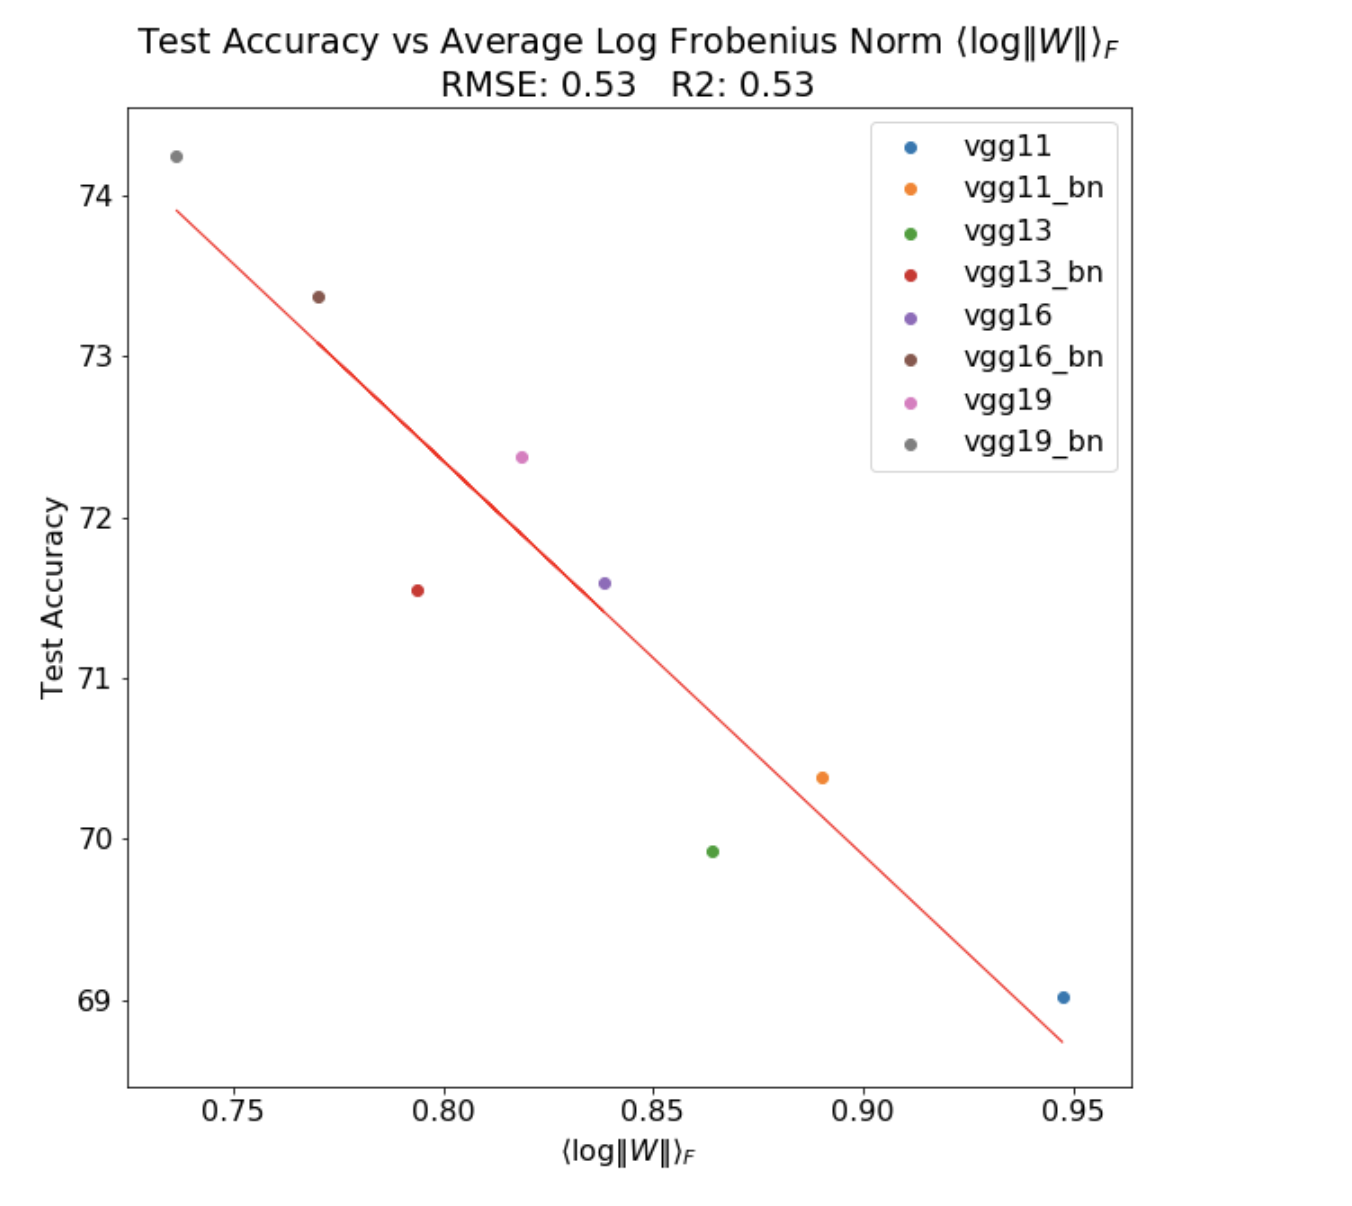
\includegraphics[width=5cm]{img/vgg-fnorm.png}
        \label{fig:vgg-fnorm}
    }
    \qquad
    \subfigure[ Spectral Norm ]{
        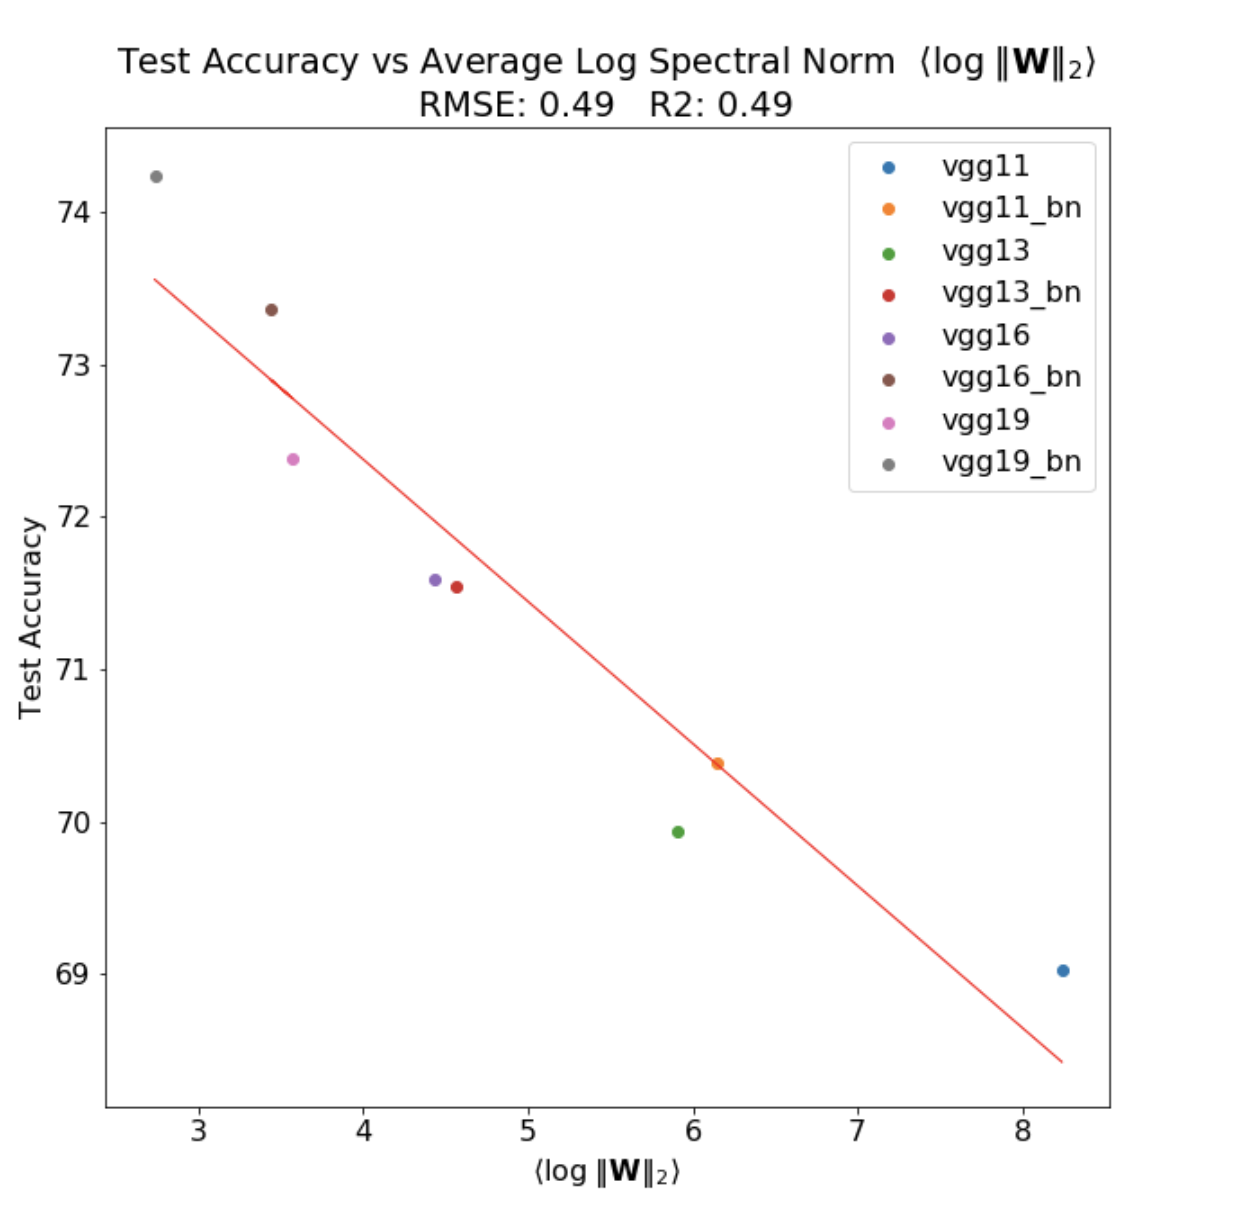
\includegraphics[width=4.9cm]{img/vgg-snorm.png}
        \label{fig:vgg-snorm}
    }
    \qquad
    \subfigure[ Weighted Alpha ]{
        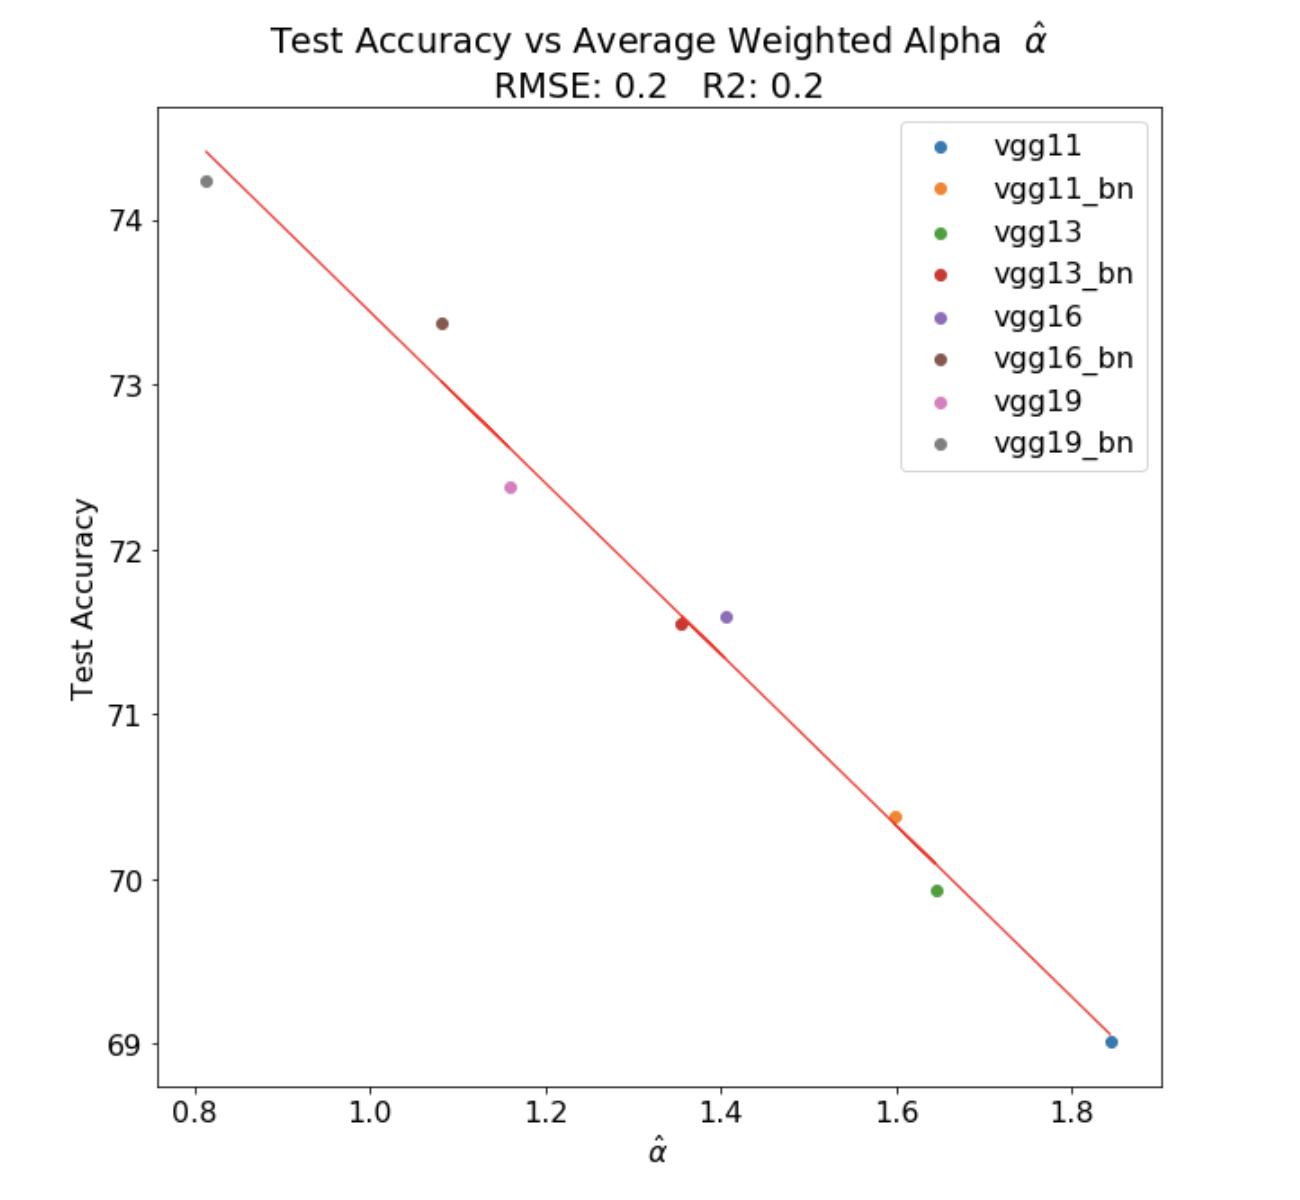
\includegraphics[width=4.9cm]{img/vgg-walpha.png}
        \label{fig:vgg-walpha}
    }
    \qquad
    \subfigure[ Alpha-Norm ]{
        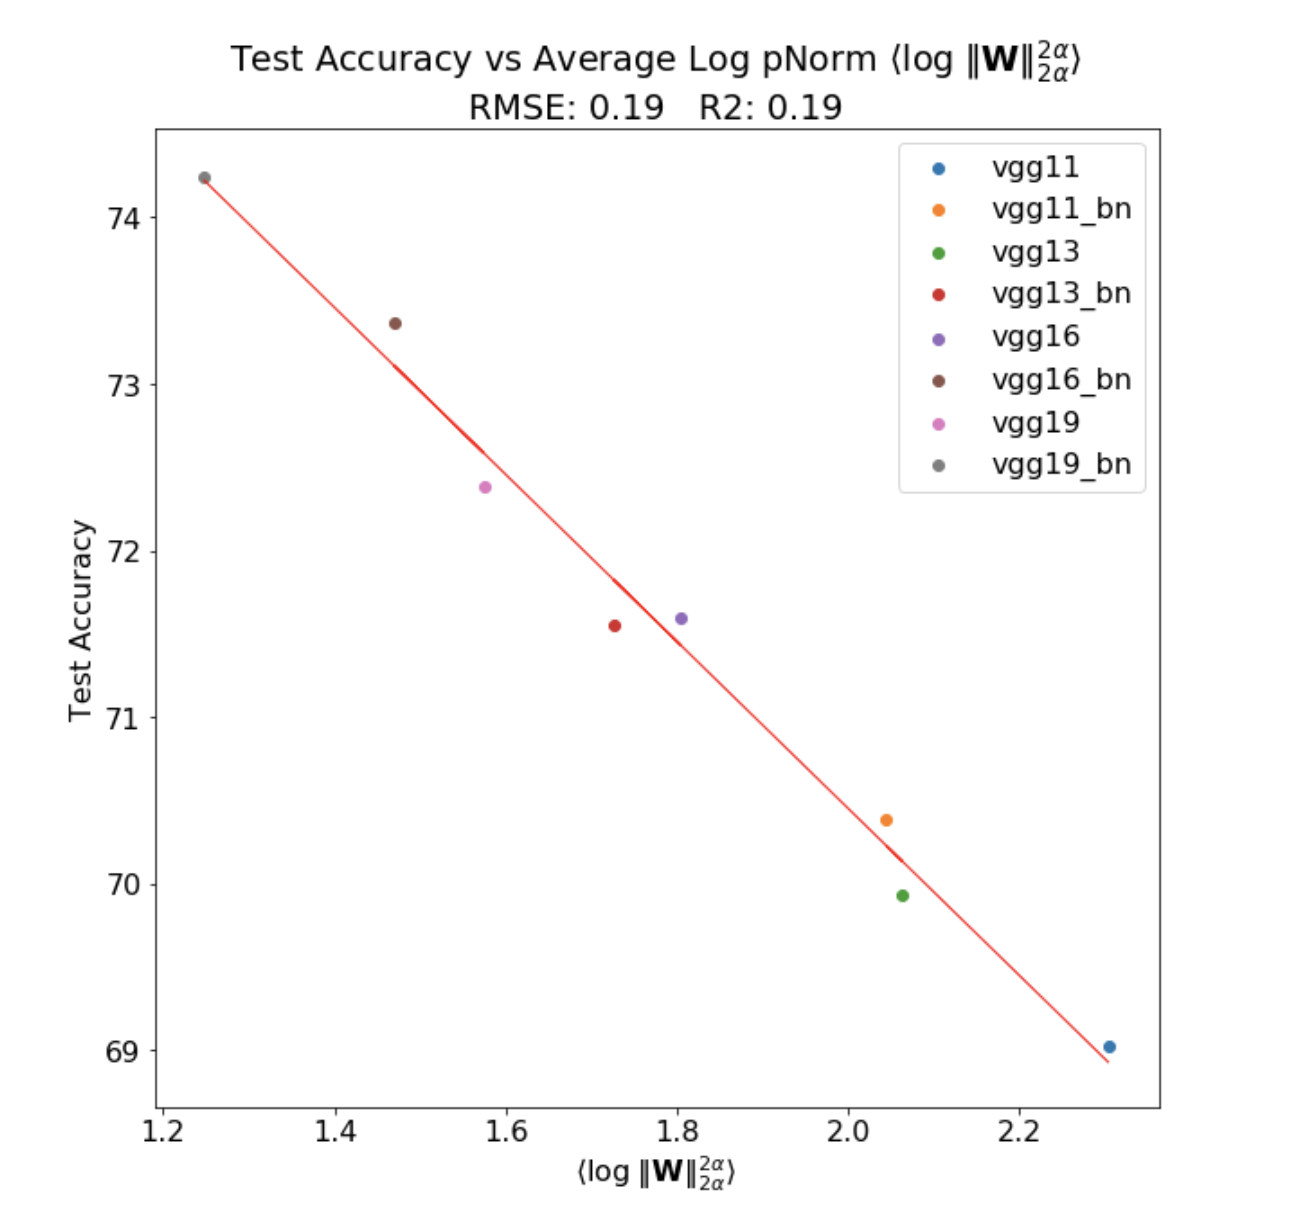
\includegraphics[width=4.9cm]{img/vgg-pnorm.png}
        \label{fig:vgg-pnorm}
    }
    \caption{Comparison of norm metrics vs reported test accuracy for pretrained VGG models, trained on ImageNet, available in pyTorch.  Plots will be updated and replace }
    

    \label{fig:vgg-metrics}
\end{figure}


VGG works remarkably well

ResNet is also correlated, but the RMSE is much larger, and 2/5 of the models are almost outliers
But note that the PyTorch distribution only has a few models.
The ResNet results look better when considering all ResNet models, trained on ImageNet1K.

ADD PLOTS FOR


\begin{figure}[t]
    \centering

    \subfigure[ ResNet ]{
        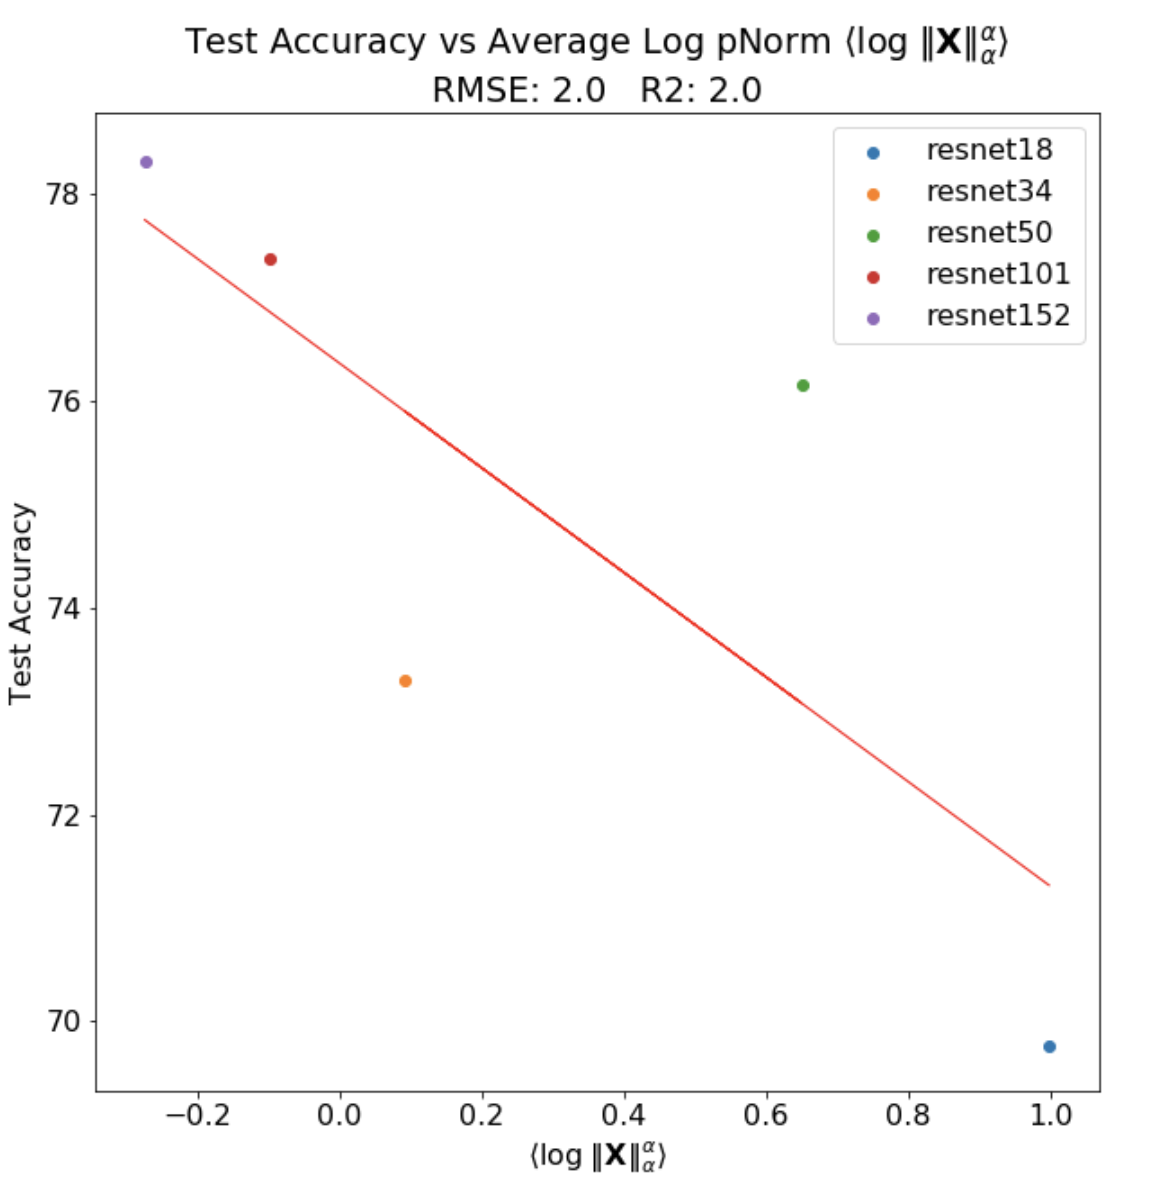
\includegraphics[width=4.2cm]{img/resnet-accuracy.png}
        \label{fig:resnet-accuracy}
    }
    \qquad
    \subfigure[ ResNet-1K ]{
        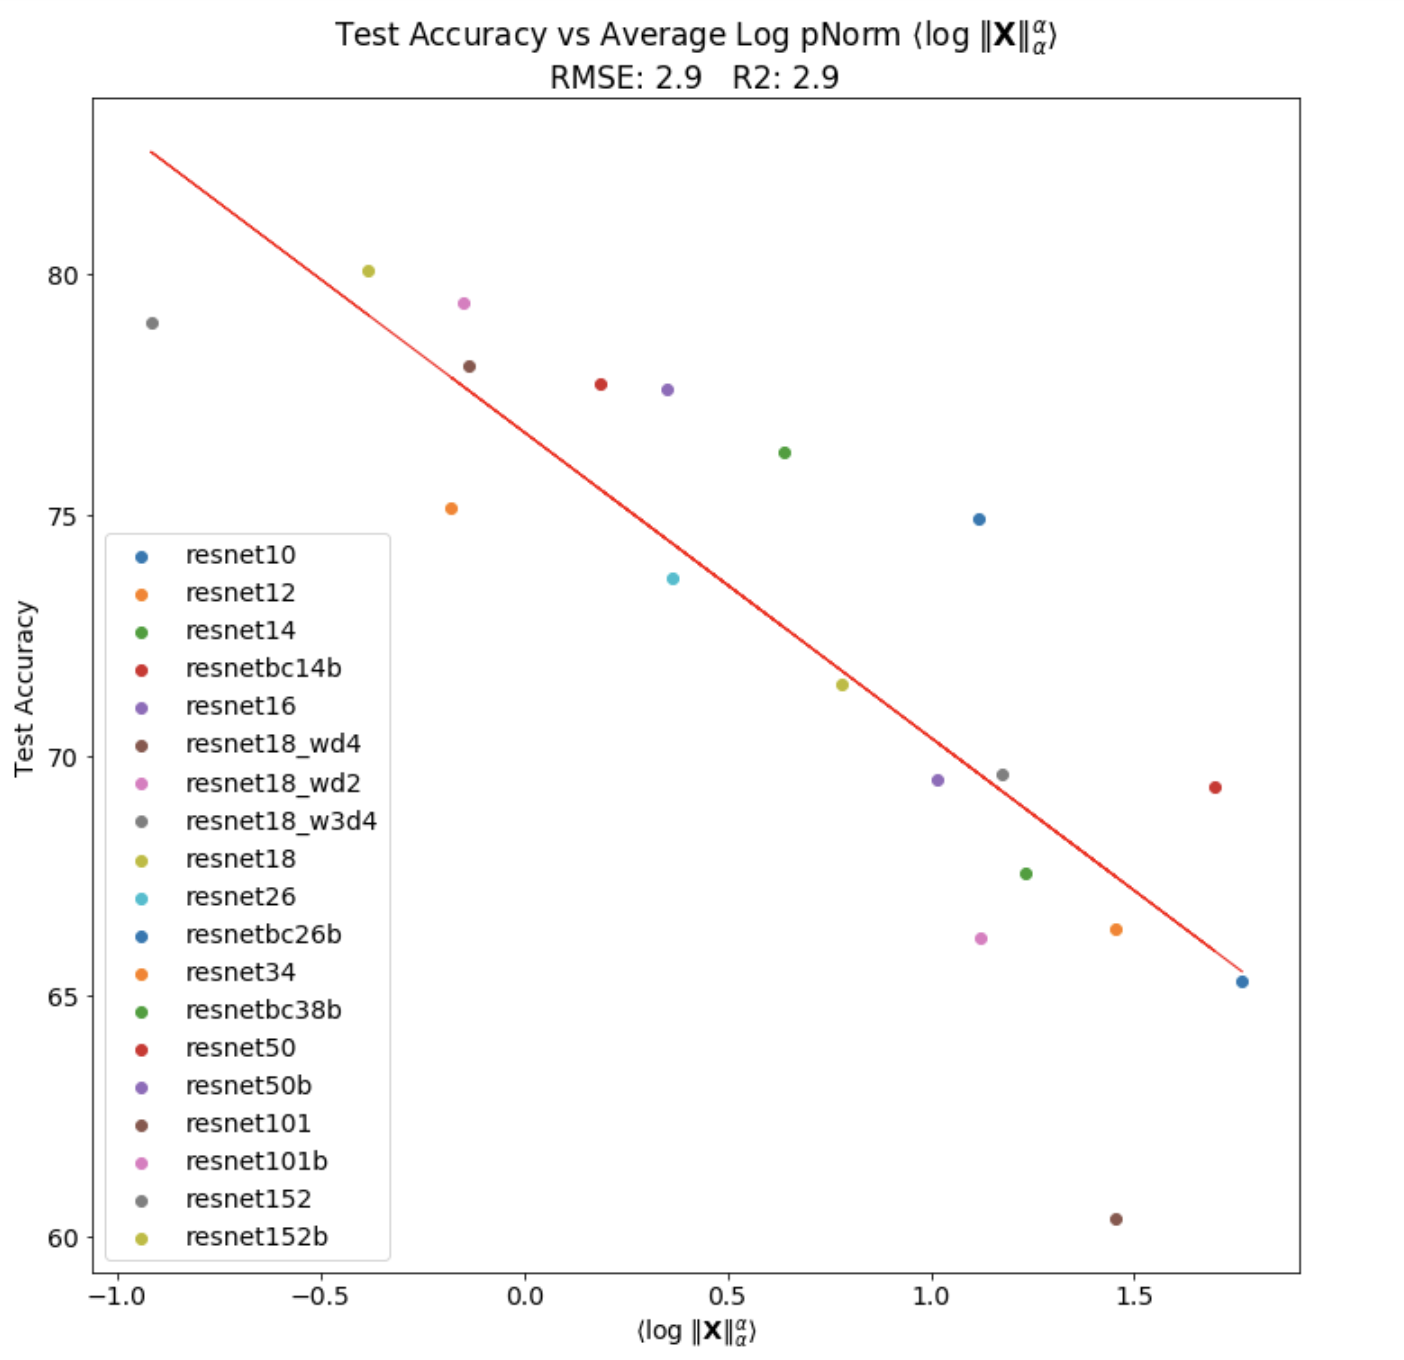
\includegraphics[width=4.5cm]{img/resnet1k-accuracy.png}
        \label{fig:resnet1k-accuracy}
    }
    \qquad
    \subfigure[ DenseNet ]{
        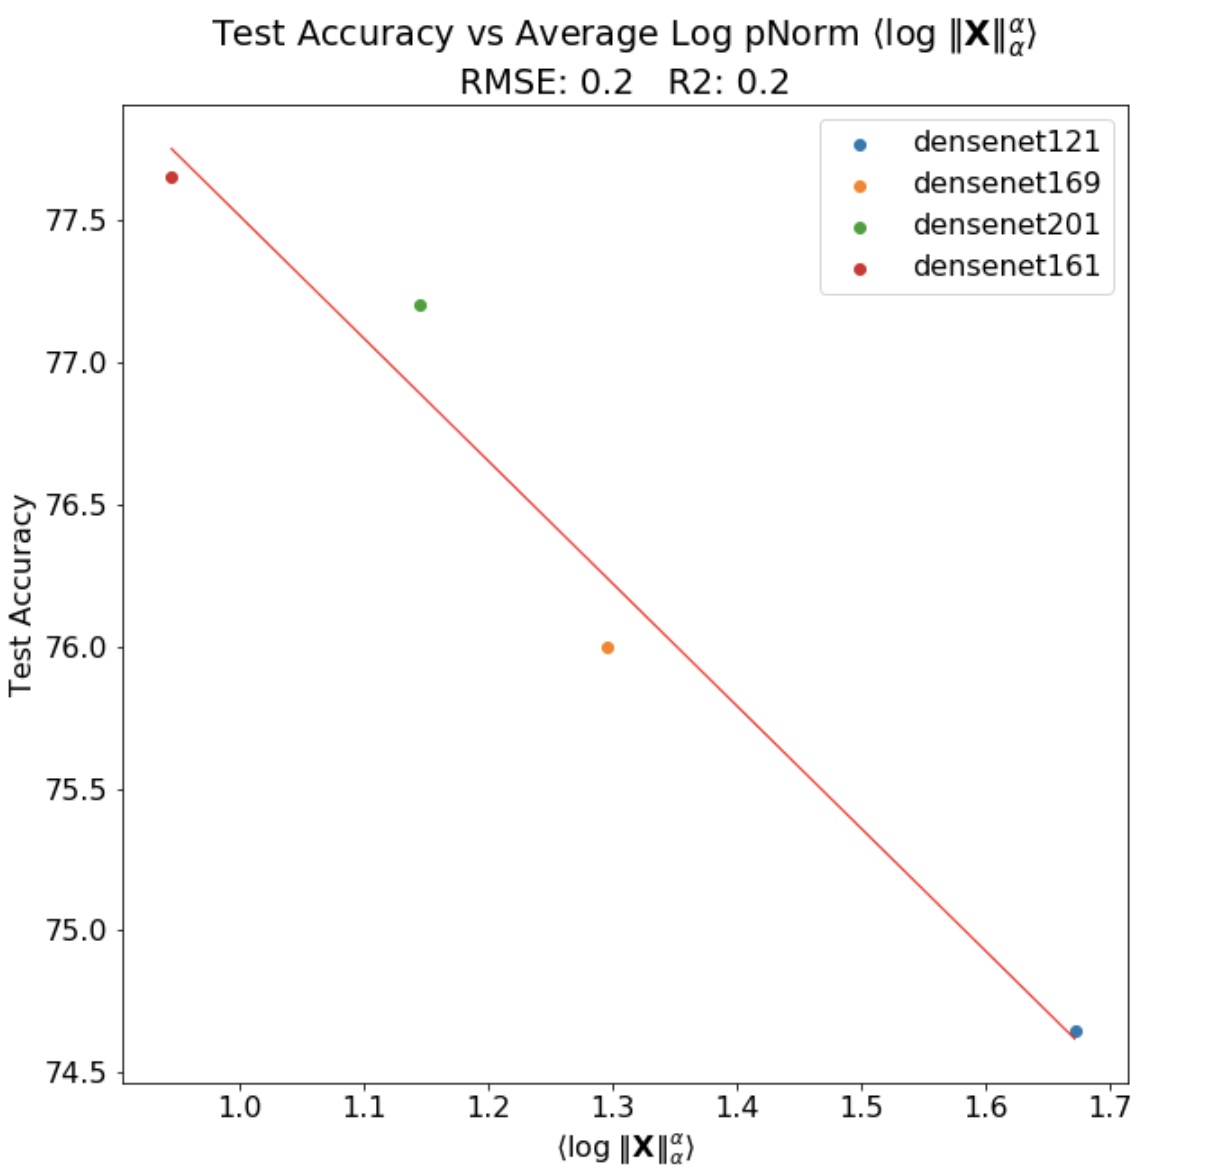
\includegraphics[width=4.4cm]{img/densenet-accuracy.png}
        \label{fig:densenet-accuracy}
    }
    \caption{$\alpha$-Norm vs reported Top1 Error for  ResNet, ResNet-1K, and DenseNet models}
    \label{fig:cv2-accuracy}
\end{figure}


TODO:  add table of metrics for these 3 models, show that alpha-Norm is best again!

\begin{table}[t]
\small
\begin{center}
\begin{tabular}{|p{1in}|c|c|c|c|c|}
\hline
   &    & Frobenus Norm & Spectral Norm & Weighted Alpha & Alpha-Norm \\
 Series & \#Models   & $\Vert\mathbf{W}\Vert_{F}$ & $\Vert\mathbf{W}\Vert_{\infty}$ & $\hat{\alpha}=\alpha\log\lambda_{max}$ & $\Vert\mathbf{X}\Vert^{\alpha}_{\alpha}$ \\
\hline
 VGG & & & & \\
 ResNet & & & & \\
 ResNet-1K & & & & \\
 DenseNet & & & & \\
\hline
\end{tabular}
\end{center}
\caption{RMSE for Linear Fits of Metric to Reported Top1 Test Error for all pre-trained models in the architecture series.  All models trained on ImageNet except ResNet-1K, which was trained on ImageNet-1K. }
\label{table:models}
\end{table}



\paragraph{Correlations and Information Flow in CV Models}

Compare VGG, ResNet, and DenseNet in the context of how many connections that have

\begin{figure}[t]
    \centering

    \subfigure[ VGG ]{
        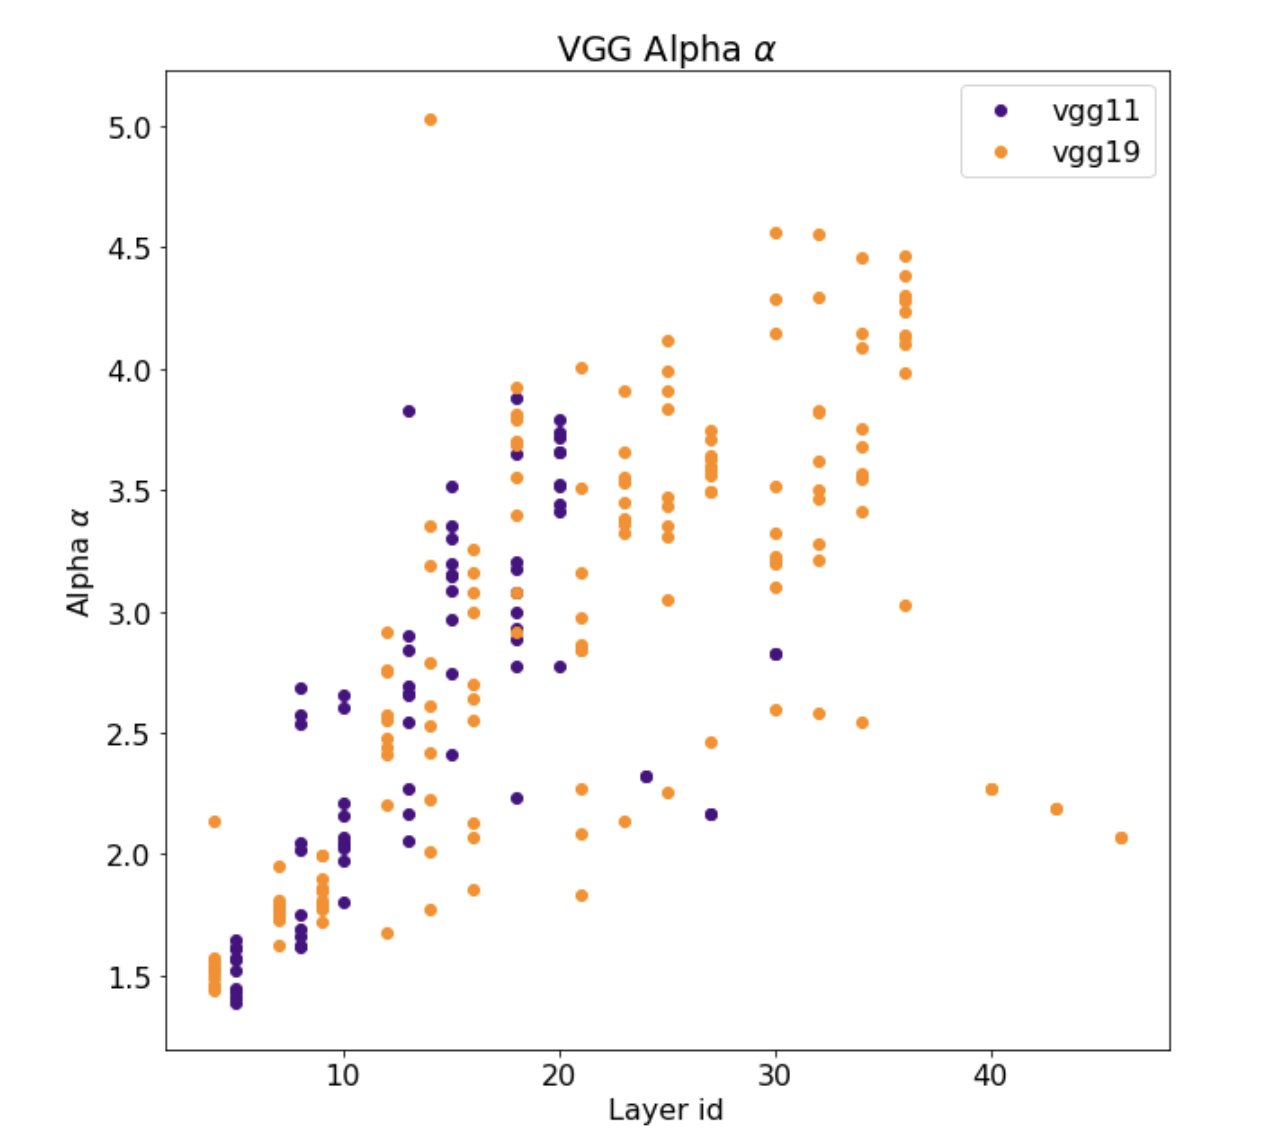
\includegraphics[width=4.1cm]{img/vgg-alpha-layers.png}
        \label{fig:vgg-alpha-layers}
    }
    \qquad
    \subfigure[ ResNet ]{
        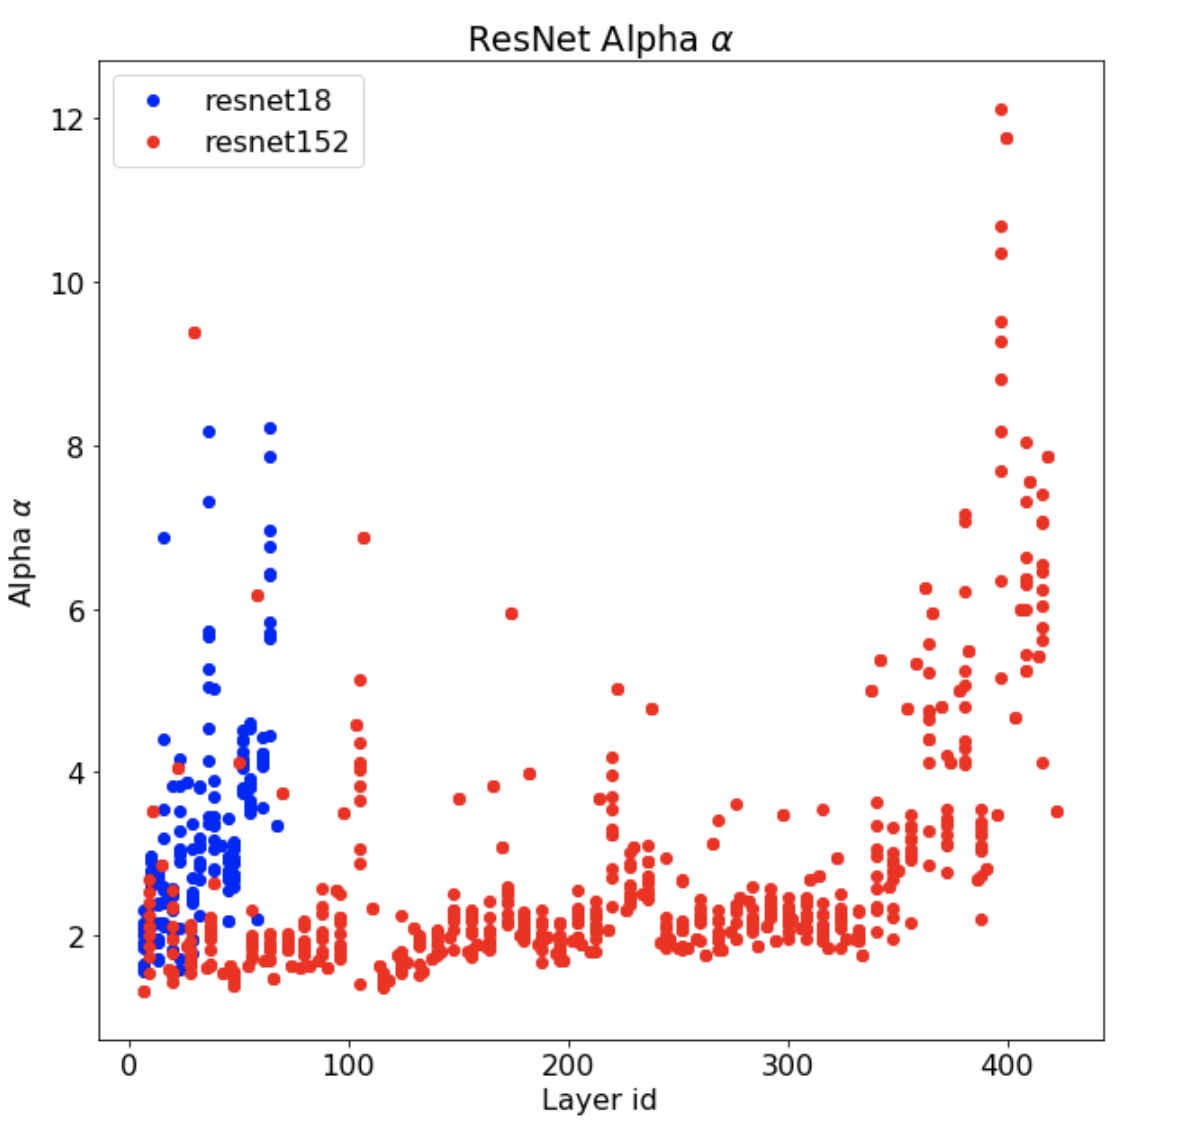
\includegraphics[width=3.8cm]{img/resnet-alpha-layers.png}
        \label{fig:resnet-alpha-layer}
    }
    \qquad
    \subfigure[ DenseNet ]{
        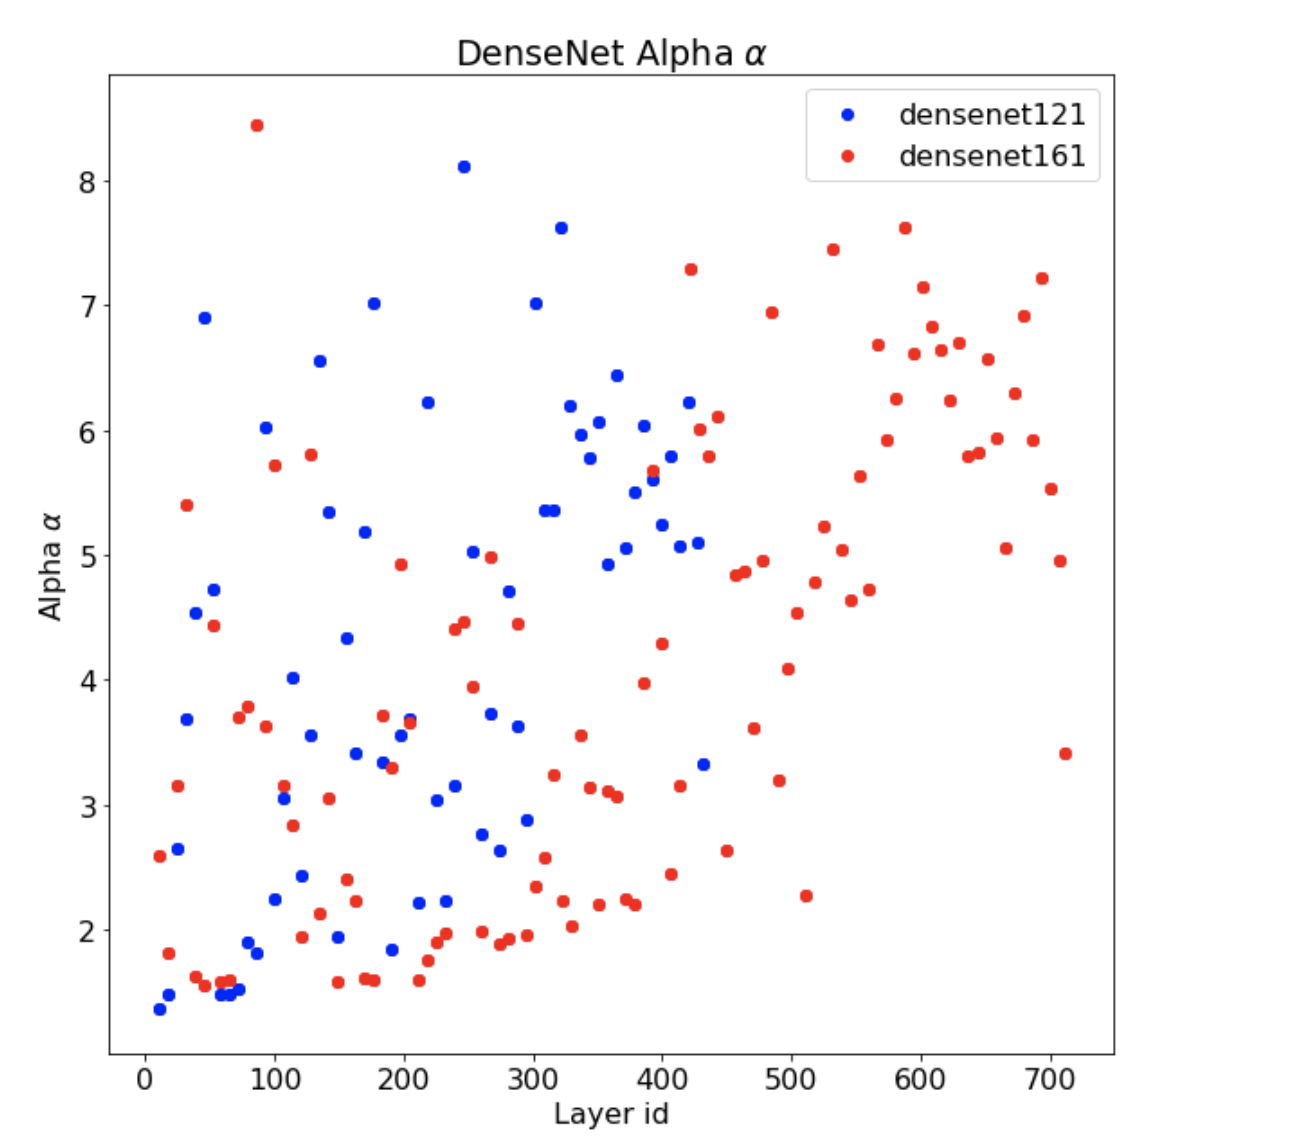
\includegraphics[width=4.1cm]{img/densenet-alpha-layers.png}
        \label{fig:densenet-alpha-layer}
    }
    \caption{Power law exponent $\alpha$ vs layer for VGG, ResNet, and DenseNet models}
    \label{fig:vgg-alpha-layers}
\end{figure}



\section{Comparison of NLP Transformer Models}
\label{sxn:nlp}

[THESE RESULTS HAVE TO BE REDONE BY REMOVING THE FIRST LAYER...]

In the past two years, nearly 100 open source, pre-trained DNNs for Natural Language Processing (NLP) have emerged,
based on the revolutionary Transformer architecture, including variants of BERT, Transformer-XML, GPT, etc.
The Transformer architectures consist of blocks of Attention layers, containing of 2 large, Feed Forward (Linear)
weight matrics \cite{Attn2017}. In contrast to the smaller pre-Activation maps arising in Cond2D layers,
the Attention matrices are significantly larger, and frequently under-correlated, with generally larger
Heavy Tailed Power Law exponents $\alpha$ (when fitting the ESD).  Here, we breifly look at a few
popular pretrained NLP DNNs to demonstrate that the Theory of Heavy Tailed Self-Regularization also
applies to NLP models and not just CV models, and to highlight how to use the theory to identify
poorly trained models where the empirical norm metrics will perform poorly.

\paragraph{OpenAI GPT Models}
We use the \emph{WeightWatcher} tool to analyze the OpenAI GPT and GPT2 models, which gives us
the opportunity to analyze the effect of both training the same model with different size data sets,
and increasing sizes of both the data set and architectures.
These models have generated significant media attention because of their remarkable ability to
 generate fake text that appears to be real and the potential misuse of this.
For this reason, the original GPT model was trained on on a deficient data set, rendering
the model interesting but not fully functional.  Later, OpenAI released a much improved model--
GPT2 (small)--which has the same architecture and number of layers as GPT, but has
been trained on a larger and betterd data set (and with other changes), making it
remarkably good at generating (near) human-quality fake text.  
By comparing GPT and GPT2, we can indentify empirical markers indicating that
a model has been poorly trained and may perform poorly when deployed.

\charles{more here ?}
We analyze GPT models deployed with the popular HuggingFace PyTorch library.
GPT has 12 layers, with 4 Multi-head Attention Blocks, giving $48$ Layer Weight Matrices $\mathbf{W}$.
Each Block has 2 components, the Self Attention (attn) and the Projection (proj) matrics.  
The self-attention  matrices are larger, of dimension ($2304\times 768$) or ($3072\times 768$).
The projection layer concatenates the self-attention results into a vector (of dimension $768$).
This gives $50$ large, typically sparse weight matrices, and they can be
 \emph{poorly correlated} when trained with insufficient data--as we shall see below.

Because GPT and GPT are trained on different data sets, the initial Embedding matrices differ in shape.
GPT  has an initial Token and Positional Embedding layers, of dimension
$(40478\times 768)$ and $(512\times 768)$, resp, whereas GPT2 has input Embeddings of shape
$(50257\times 768)$ and $(1024\times 768)$, resp.  Interstingly, they also have very spectral properties,
also shown below.

The additional OpenAI GPT2 (English) models are: \emph{gpt-medium, got-large, and gpt-xl}, 
having include $12, 24, 36, and 48$ layers, resp., with increasingly larger weight matrices.
The model card for GPT2 is published on github.\footnote{\url{https://github.com/openai/gpt-2/blob/master/model_card.md}}.
Table \ref{table:nlp} reports results for the average log norm metrics, using \emph{weightwatcher (0.2.7)},
and with fully reproducible Jupyter notebooks.\footnote{\url{https://github.com/CalculatedContent/kdd2020}}


\begin{table}[t]
\small
\begin{center}
\begin{tabular}{|p{1in}|c|c|c|c|c|}
\hline
   &    & Frobenius Norm & Spectral Norm & Weighted Alpha & Alpha-Norm \\
 Series & \#Layers   & $\Vert\mathbf{W}\Vert_{F}$ & $\Vert\mathbf{W}\Vert_{\infty}$ & $\hat{\alpha}=\alpha\log\lambda_{max}$ & $\Vert\mathbf{X}\Vert^{\alpha}_{\alpha}$ \\
\hline
 GPT & & & & &\\
GPT2 & 50 & 2.05 &2.59& 9.78 & 10.03 \\
GPT2 medium & 98 & 2.08 &2.58& 9.74 & 10.01 \\
GPT2 large & 146 & 1.85 &1.99& 7.67 & 7.94 \\
GPT2 xl & 194 & 1.86 &1.92& 7.17 & 7.51 \\
\hline
\end{tabular}
\end{center}
\caption{Average Log Norm Metrics for pretrainnd OpenAI GPT and GPT2 models.}
\label{table:nlp}
\end{table}

Explain why Log Norm is sooo large...alpha is off may need to prune the alpha

\paragraph{The Heavy Tailed Power Law Exponents in GPT and GPT2}

are very differenmt, with GPT2 having both a notably smaller mean $\alpha$, and far fewer, unusually large outliers.
Figure \ref{fig:gpt-alphs-hist} shows the empirical density (histogram) of $\alpha$
for all layers in GPT (blue) and GPT2 (red).  \charles{discuss more}

\begin{figure}
    \centering
    \subfigure[Power Law Exponent $\alpha$]{
        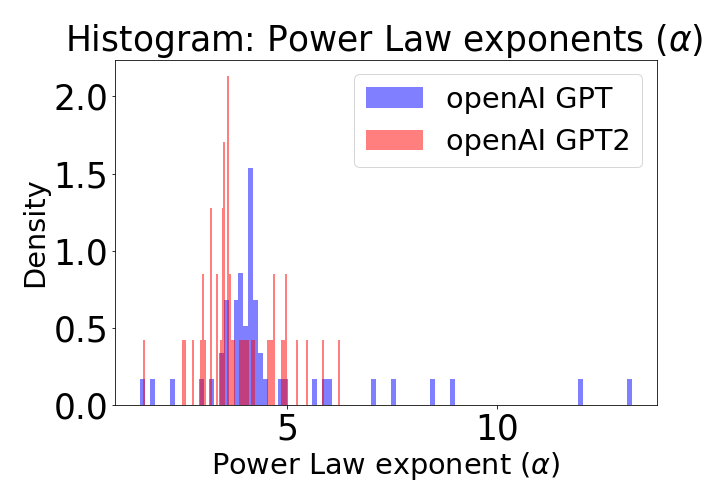
\includegraphics[width=5cm]{img/GPT-alpha-hist.png}
        \label{fig:GPT-alpha.hist.png}
       }
    \qquad
    \subfigure[Log Spectral Norm $\log\Vert\mathbf{W}\Vert_{\infty}$]{
        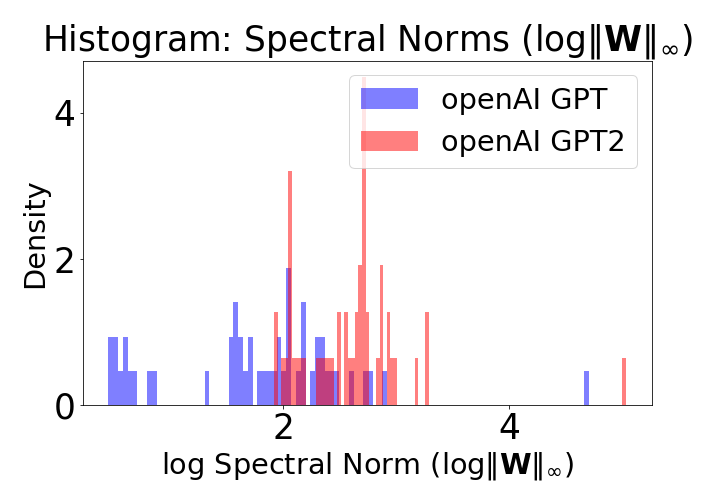
\includegraphics[width=5cm]{img/GPT-snorm-hist.png}
        \label{fig:GPT-snorm.hist.png}
       }


   \caption{Comparison of Heavy Tailed Power Law exponents $\alpha$, and log Spectral Norms $\log\Vert\mathbf{W}\Vert_{\infty}$
for the OpenAI GPT and GPT2 (small) pretrained models.}

\end{figure}

\charles{We have redo the spectral norm and remove the outliers}

\paragraph{The Correlation Flow in GPT and GPT2} also differs significantly between GPT and GPT2.
Figure \ref{fig:gpt-alpha-layer} plots $\alpha$ vs the layer id for each model.


\charles{Discuss Spectral Norm, alpha-Norm}

\begin{figure}[t]
    \centering

    \subfigure[ Power Law Exponent $\alpha$  ]{
        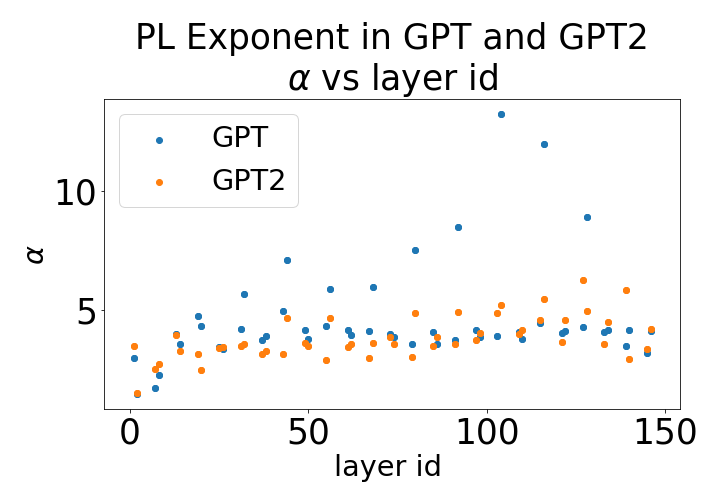
\includegraphics[width=4.5cm]{img/GPT-alpha-depth.png}
        \label{fig:gpt-alpha-layer}
    }
    \qquad
    \subfigure[ Spectral Norm $\Vert\mathbf{W}\Vert_{\infty}$]{
        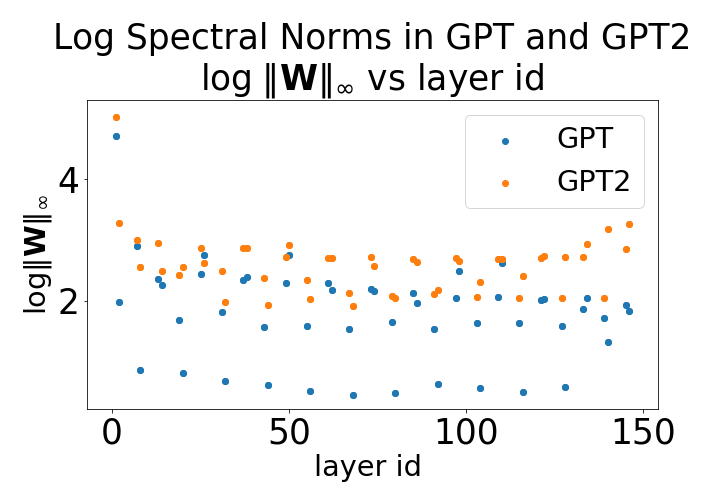
\includegraphics[width=4.5cm]{img/GPT-snorm-depth.png}
        \label{fig:resnet-snorm-layer}
    }
    \qquad
    \subfigure[ Alpha-Norm $\Vert\mathbf{X}\Vert_{\alpha}^{\alpha}$]{
        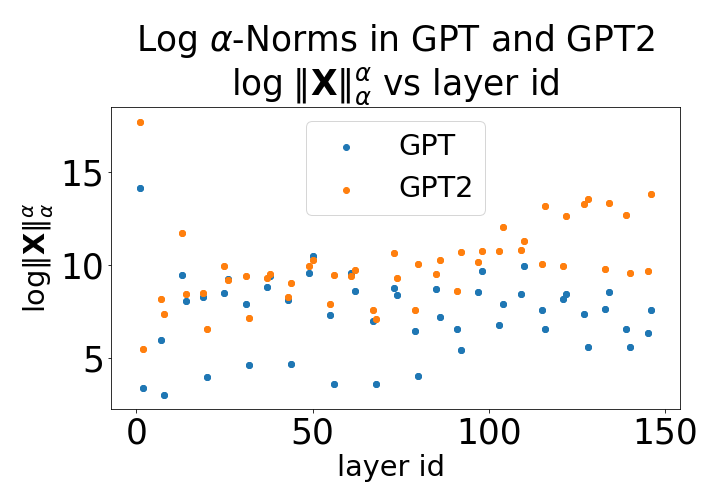
\includegraphics[width=4.5cm]{img/GPT-pnorm-depth.png}
        \label{fig:gpt-pnorm-layer}
    }
    \caption{Comparison of Correlation Flow and Spectral Norm for OpenAI GPT and GPT2   }
    \label{fig:gpt-alpha-layers}
\end{figure}

\paragraph{GPT2: small, medium, large, extra-large} 

Figure \ref{fig:gpt-alpha-layers} ...

For this series of GPT2 models, the average $\alpha$ still decreases with increasing model size,
althogh, the differences are less noticible than between the GPT and GPT2 models.
Unlike GPT, however, the Layer Spectral Norms $\vert\mathbf{W}\Vert_{\infty}$ 
and Alpha-Norms $\vert\mathbf{W}\Vert_{\alpha}^{\alpha}$
 behave  as expected for GPT2 layers, with the larger models 
consistently having  smaller norms. 

\begin{figure}[t]
    \centering

    \subfigure[ Power Law Exponent $\alpha$  ]{
        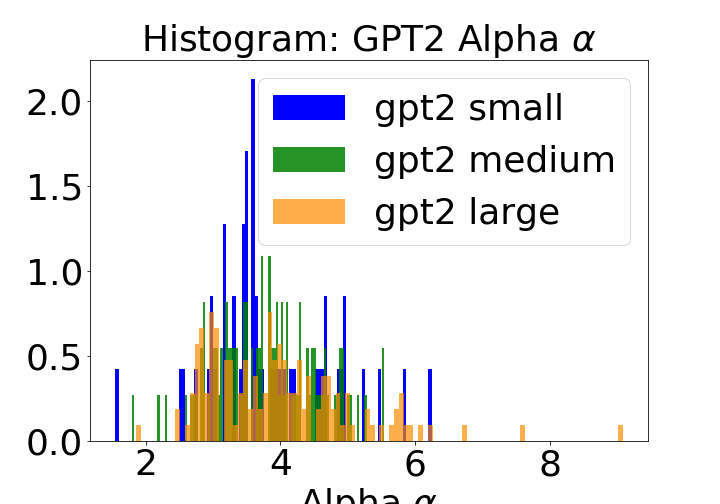
\includegraphics[width=4.5cm]{img/GPT2_all_alpha_hist.png}
        \label{fig:gpt-alpha-layer}
    }
    \qquad
    \subfigure[ Spectral Norm $\Vert\mathbf{W}\Vert_{\infty}$]{
        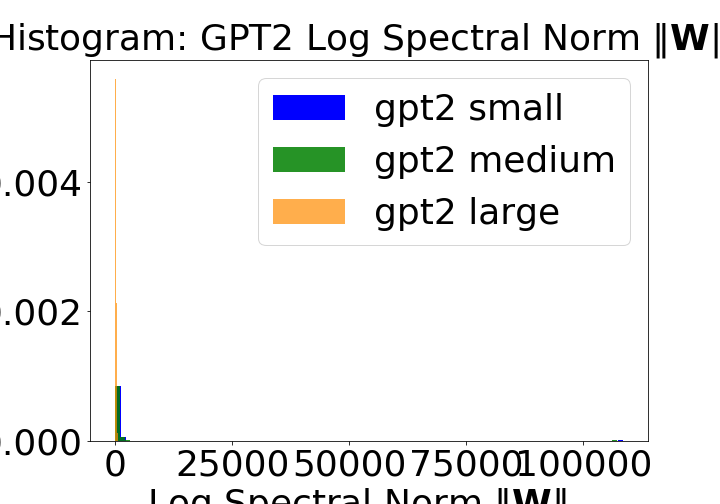
\includegraphics[width=4.5cm]{img/GPT2_all_spectralnorm_hist.png}
        \label{fig:resnet-snorm-layer}
    }
    \qquad
    \subfigure[ Alpha-Norm $\Vert\mathbf{X}\Vert_{\alpha}^{\alpha}$]{
        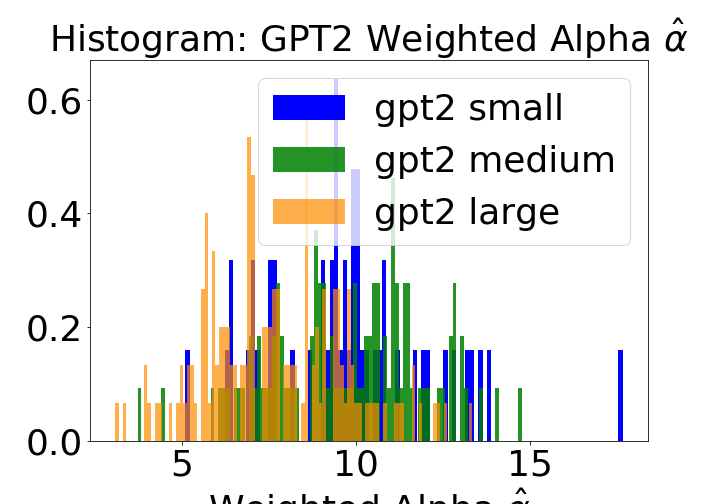
\includegraphics[width=4.5cm]{img/GPT2_all_alpha_weighted_hist.png}
        \label{fig:gpt-pnorm-layer}
    }
    \caption{Comparison of Power Law Exponnents, Spectral Norm, and Alpha-Norm for different size models in the GPT2 architecture series.  Spectral Norm dhistogram does not contain the first 2 layers because the values are unusually large.}
    \label{fig:gpt-alpha-layers}
\end{figure}





%KDD% 
\vspace{-1mm}
\section{Comparing Hundreds of Models}
\label{sxn:all_cv_models}
%\vspace{-1mm}

In this section, we summarize results from a large-scale analysis of hundreds of publicly-available  models, including models developed for image 
classification, segmentation, and a range of related tasks.  
Our aim is to provide a broad analysis that complements the detailed analysis in Sections~\ref{sxn:cv} and~\ref{sxn:nlp}.
There, we considered CV and NLP models with similar structures. 
Here, we provide much broader conclusions based on a much larger set of models with a much more diverse set of structures. % about norm-based and PL-based metrics.
The models we consider have been pretrained on nine datasets.   %, shown in Table~\ref{table:datasets}.
%including ImageNet-1K, and CIFAR-10, CIFAR-100, Street View House Numbers (SVHN), Caltech-UCSD Birds-200-2011 (CUB-200-2011), Pascal VOC2012, ADE20K, Cityscapes, and Common Objects in Context (COCO). 
%%The pretrained models and their accuracy metrics are summarized in the osmr github~\cite{charles-add-link}.
We provide full details about how to reproduce these results in Appendix~\ref{sxn:appendix}.

\begin{table}[t]
\small
\begin{center}
\begin{tabular}{|p{1in}|c|c|c|c|}
%KDD% \begin{tabular}{|p{0.75in}|c|c|c|c|}
\hline
%    & Frobenius Norm & Spectral Norm & Weighted Alpha & Alpha-Norm \\
%    & $\langle\log\Vert\mathbf{W}\Vert_{F}\rangle$ & $\langle\log\Vert\mathbf{W}\Vert_{\infty}\rangle$ & $\langle\hat{\alpha}=\alpha\log\lambda_{max}\rangle$ & $\langle\log\Vert\mathbf{X}\Vert^{\alpha}_{\alpha}\rangle$ \\
Series        & $\log\Vert\cdot\Vert_{F}$ & $\log\Vert\cdot\Vert_{\infty}$ & $\hat{\alpha}$ & $\log\Vert\cdot\Vert^{\alpha}_{\alpha}$ \\
\hline
$R^{2}$ (mean) & 0.63 &  0.55 & \textbf{0.64} & \textbf{0.64} \\
$R^{2}$ (std)  & 0.34 &  0.36 & \textbf{0.29} &          0.30 \\
\hline
$MSE$ (mean)   & 4.54 &  9.62 &          3.14 & \textbf{2.92} \\
$MSE$ (std)    & 8.69 & 23.06 &          5.14 & \textbf{5.00} \\
\hline
\end{tabular}
\end{center}
\caption{Comparison of linear regression fits for different average Log Norm and Weighted Alpha metrics across 5 CV datasets, 17 architectures, covering 108 (out of over 400) different pretrained DNNs.  
         We include regressions only for architectures with five or more data points, and which are positively correlated with test error.
         These results can be readily reproduced using the Google Colab notebooks (see Appendix~\ref{sxn:appendix}). 
        }
\label{table:results}
\end{table}


We choose ordinary least squares (OLS) regression to quantify the relationship between quality metrics (computed with the \emph{WeightWatcher} tool) 
and the reported test error and/or accuracy metrics.
We regress the metrics on the Top1 (and Top5) reported errors (as dependent variables).
These include Top5 errors for the ImageNet-1K model, percent error for the CIFAR-10/100, SVHN, CUB-200-2011 models, and Pixel accuracy
(Pix.Acc.) and Intersection-Over-Union (IOU) for other models.
We regress them individually on each of the norm-based and PL-based metrics, as described in Section~\ref{sxn:cv}.

Our results are summarized in Table~\ref{table:results}.
For the mean, larger $R^{2}$ and smaller $MSE$ are desirable; and for the standard deviation, smaller values are desirable.
Taken as a whole, over the entire corpus of data, PL-based metrics are somewhat better for both the $R^{2}$ mean and standard deviation;
and PL-based metrics are much better for $MSE$ mean and standard deviation.
These (and other) results suggest our conclusions from Sections~\ref{sxn:cv} and~\ref{sxn:nlp} hold much more generally, and they suggest
obvious questions for future work.


%KDD% \vspace{-1mm}
\section{Conclusion}
\label{sxn:conc}
%\vspace{-1mm}

We have developed (based on strong theory) and evaluated (on a large corpus of publicly-available pretrained models from CV and NLP) methods to predict trends in the quality of state-of-the-art neural networks---without access to training or testing data.
Prior to our work, it was not obvious that norm-based metrics would perform well to predict trends in quality \emph{across} models (as they are usually used \emph{within} a given model or parameterized model class, e.g., to bound generalization error or to construct regularizers).
Our results are the first to demonstrate that they can be used for this important practical problem.
That PL-based metrics perform better (than norm-based metrics) should not be surprising---at least to those familiar with the statisical mechanics of heavy tailed and strongly correlated systems~\cite{BouchaudPotters03, SornetteBook, BP11, bun2017} (since our use of PL exponents is designed to capture the idea that well-trained models capture correlations over many size scales in the data).
Again, though, our results are the first to demonstrate this.
It is also gratifying that this approach can be used to provide fine-scale insight (such as rationalizing the flow of correlations or the collapse of size scale) throughout a network. 

We conclude with a few comments on what a \emph{practical theory} of DNNs should look like.
To do so, we distinguish between two types of theories:
\emph{non-empirical or analogical theories}, in which one creates, often from general principles, a very simple toy model that can be analyzed rigorously, and one then argues that the model is relevant to the system of interest; and 
\emph{semi-empirical theories}, in which there exists a rigorous asymptotic theory, which comes with parameters, for the system of interest, and one then adjusts or fits those parameters to the finite non-asymptotic data.
A drawback of the former approach is that it typically makes very strong assumptions on the data, and the strength of those assumptions can limit the practical applicability of the theory.
Much of the work on the theory of DNNs focuses on the former type of theory.
Our approach focuses on the latter type of theory.
Our results, which are based on our \emph{use} of sophisticated statistical mechanics theory to solve important practical DNN problems, suggests that our approach should be of interest more generally for those interested in developing a practical DNN theory.




\vspace{-2mm}
\noindent
\paragraph{Acknowledgements.}
MWM would like to acknowledge ARO, DARPA, NSF, and ONR as well as the UC Berkeley BDD project for providing partial support of this work.
We would also like to thank Amir Khosrowshahi and colleagues at Intel for helpful discussion regarding the Group Regularization distillation technique.

\bibliographystyle{unsrt}
%\bibliographystyle{plain}
{\small
%\bibliography{gen_gap}
\bibliography{dnns}
%\bibliography{dnns,gen_gap}
}

\appendix
\section{Appendix}

XXX.  APPENDIX.


\end{document}
